\section{Introduction}


\subsection{Overview}

Edges in real-world networks are often directed, such as links on the world wide web, follows on Twitter or disease transmission. When analysing networks a natural quantity to consider is are the degrees of nodes in the network.  In this paper we will consider sampling an i.i.d.\ sequence of in- and out-degrees. Conditional on the total in-degree being equal to the total out-degree, we will sample a uniform directed graph (digraph) with the given degree sequence. Results on such graphs provide insight into what additional structure a real-world network has beyond it's degree sequence.

When considering such models, previous work by \citet{cooperSizeLargestStrongly2004} shows that there is a phase transition in the directed connectivity of the graph. Below some threshold, each of the strongly connected components of the graph will contain a negligible proportion of vertices in the graph whereas above the threshold there will exist a unique strongly connected component that occupies a positive proportion of the vertices.  We will study the behaviour of the model at criticality, specifically that there exists a sequence of random weighted directed multigraphs that can be understood as the scaling limit of the strongly connected components when viewed in decreasing order of size.

\subsection{Graph theory}

\begin{figure}
    \centering
    \includegraphics[scale=0.6]{Content/Pictures/biggraph2.pdf}
    \caption{A directed graph on [17]. The strongly connected components have vertex sets $\{1,2,5,17\}$, $\{3,6,8,9,14,16\}$, $\{7,11\}$, $\{4\}$, $\{10\}$, $\{12\}$, $\{13\}$, and $\{15\}$. Source figure: \cite{goldschmidtScalingLimitCritical2019}}
    \label{fig.SCCs}
\end{figure}

There are two notions of connectivity when working with a directed graph - weak and strong connectivity. We will be working with the strong notation. We say a vertex $v$ leads to a vertex $w$ if there exists a directed path from $v$ to $w$ in the graph. We say $v$ is strongly connected to $w$ if $v$ leads to $w$ and $w$ leads to $v$. A graph is strongly connected if any pair of vertices in the graph are strongly connected. The relation is an equivalence relation. The digraphs induced by the equivalence classes of are referred to as the strongly connected components (SCCs).

\subsection{Description of the model}

We consider $n$ vertices, to each of which we assign an in-degree and an out-degree. The degree tuples are independent and identically distributed with law $\nu$. For each $i\in [n]$, let $\mathbf{D}_i=(D^-_i,D^+_i)$ be the in- and out-degree of vertex $i$. In order for a graph with this degree sequence to exist, we require that $\sum_{i=1}^n D^-_i=\sum_{i=1}^n D^+_i$, so we will condition on this event. Conditional on $(\mathbf{D}_1,\dots,\mathbf{D}_n)$, sample a uniform digraph with this degree sequence. Denote resulting random digraph by $\vec{G}_n(\nu)$. We are interested in the limit under scaling of the strongly connected components of $\vec{G}_n(\nu)$ as $n\to \infty$.

We require the degree distribution to satisfy the following properties.

\begin{enumerate}
    % \item $\E[(D^-) + D^+)^3] < \infty$
    \item $\E[(D^-)^i(D^+)^j]< \infty$ for $1 \leq i+j\leq 3$ and for $\{i,j\}=\{1,3\}$
    \item $\E[D^-] = \E[D^+]$.
    \item \myworries{lattice condition}
\end{enumerate}

The first condition is required to ensure the steps of a random walk used in the proof has finite variance and thus will convergence (under rescaling) to a Brownian motion.

The second condition and third condition makes sure the event $\{\sum_{i=1}^n D^-_i = \sum_{i=1}^n D^+_i\}$ is well behaved. The second condition ensures this is not a large deviation event and the third condition ensures this event has positive probability for all $n \geq 1$. 

\myworries{go over criticality condition}

We define the following parameters, that will determine the behaviour of the strongly connected components in the limit.
\begin{enumerate}
    \item $\mu:=\E[D^-]=\E[D^+]=\E[D^-D^+]$
    \item $\nu_-:=\frac{\E[(D^-)^2]-\mu}{\mu}$ 
    \item $\sigma_-:=\left(\frac{\mu\E[(D^-)^3]-\E[(D^-)^2]^2}{\mu^2}\right)^{1/2}$ 
    \item $\sigma_+:=\left(\frac{\E[D^-(D^+)^2]-\mu}{\mu}\right)^{1/2}$ 
    \item $\sigma_{-+}:=\frac{\E[(D^-)^2D^+]-\E[(D^-)^2]}{\mu}$ 
\end{enumerate}
% \begin{remark}
% Conditions \ref{cond.beta} and \ref{cond.gamma} ensure that the Central Limit Theorem applies to the fluctuations of the first explored in-degrees around their mean. Condition \ref{cond.critical} ensures that the branching process corresponding to the depth-first exploration (i.e. the exploration of the out-components) is critical. Condition \ref{cond.rho} ensures that this branching process has Brownian scaling. Condition \ref{cond.tau} ensures that the covariance of the in- and out-degrees that are discovered first is finite. Condition \ref{cond.iota} ensures that the strongly connected components are $3$-regular. 
% \end{remark}
\subsection{Metric directed multigraphs and kernels}

\begin{figure}[htbp]
    \centering

    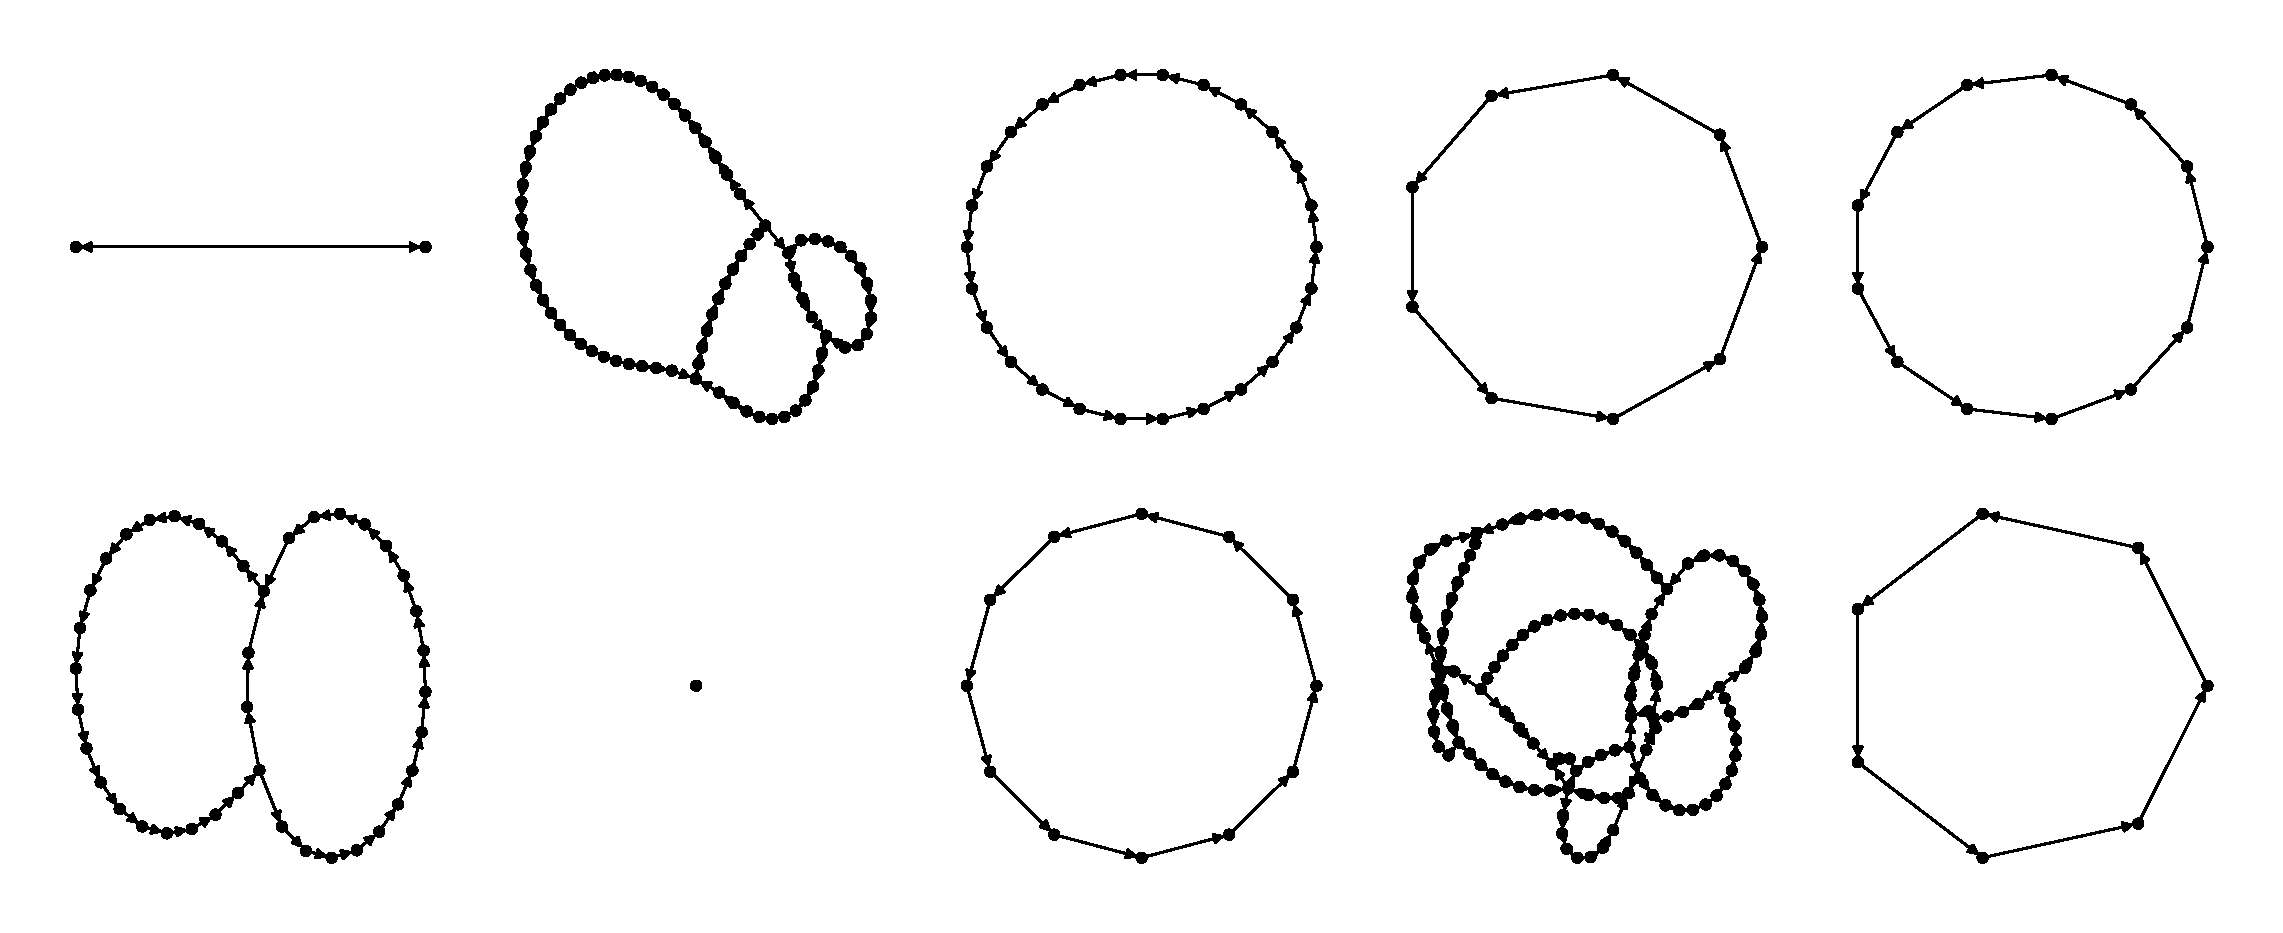
\includegraphics[width=\textwidth]{Content/Pictures/largest_sccs.eps}
    
    \caption{The largest SCC from samples of a directed configuration model with independent $\text{Poisson(1)}$ in- and out-degrees}
    \label{fig:largest-sccs}
\end{figure}

In \cref{fig:largest-sccs} we see the largest SCC from samples of a directed configuration model. As can be seen, while the lengths of paths in the SCC are long, the actual structure of the SCC is often quite simple. Previous work by \citet{goldschmidtScalingLimitCritical2019} shows this is true for the directed Erdős--Renyi model. There it was shown that while the lengths of paths in the SCC will scale like $n^{1/3}$, the actual structure of the SCC will remain finite.

To formalise this idea we will introduce metric directed multigraphs (MDMs). These are simply weighted directed multigraphs, but in our context it is more appropriate to think of the weights as lengths hence the change in naming. Formally a directed multigraph is a tuple $(V, E, r)$ where
\begin{enumerate}
    \item $V$ is a set of vertices,
    \item $E$ is a set of edges, and
    \item $r: E \to V \times V$ is a function mapping edges to their head and tail.
\end{enumerate}
Associated with $r$ are two functions $r_1: E \to V$ and $r_2: E \to V$ such that
\begin{equation*}
    r(e) = (r_1(e), r_2(e))
\end{equation*}
for all $e \in E$. $r_1(e)$ is the tail of the edge $e$ and $r_2(e)$ is the head of the edge $e$. Then a metric directed multigraph (MDM) is a tuple $M = (V, E, r, l)$ where $(V, E, r)$ is a directed multigraph and $l:E \to [0, \infty)$. Let $\zeroloop$ denote the MDM consisting of a single vertex with a self loop of length 0.

An isomorphism between two MDMs $M = (V, E, r, l)$ and $M' = (V', E', r', l)$ is a pair of functions $(i_V, i_E)$ where $i_V: V \to V'$ and $i_E: E \to E'$ are bijections satisfying
\begin{equation*}
    r'(i_E(e)) = (i_V(r_1(e)), i_V(r_2(e)))
\end{equation*}
for all $e \in E$. We say two MDMs are isomorphic if there exists an isomorphism between them. Intuitively this means the MDMS have the same graph structures up to a relabelling of the edges and vertices. Write $\iso(M, M')$ for the set of all isomorphisms between $M$ and $M'$.

We now define a distance $\distmdm$ between two MDMs $M$ and $M'$.  Any isomorphism between $M$ and $M'$ gives a correspondence between the edges of $M$ and the edges of $M'$. We can then take an $\ell_{\infty}$ distance between the lengths of the edges and finally take the isomorphism which minimizes this distance. If $M$ and $M'$ are not isomorphic we can set the distance to be infinite. Formally
\begin{equation*}
    \distmdm(M, M') = \begin{cases}
        \inf_{(i_V, i_E) \in \iso(M, M')} \sup_{e \in E} \abs{l(e) - l(i_E(e))} & \text{if $M$ and $M'$ are isomorphic,} \\
        \infty & \text{otherwise.}
    \end{cases}
\end{equation*}

\begin{figure}[htbp]
    \centering
    \begin{subfigure}[htbp]{0.45\textwidth}
        \centering
        \includegraphics[width=0.95\textwidth]{Content/Pictures/smoothing1.eps}
        \caption{The graph before smoothing $w$}
    \end{subfigure}
    \hfill
    \begin{subfigure}[htbp]{0.45\textwidth}
        \centering
        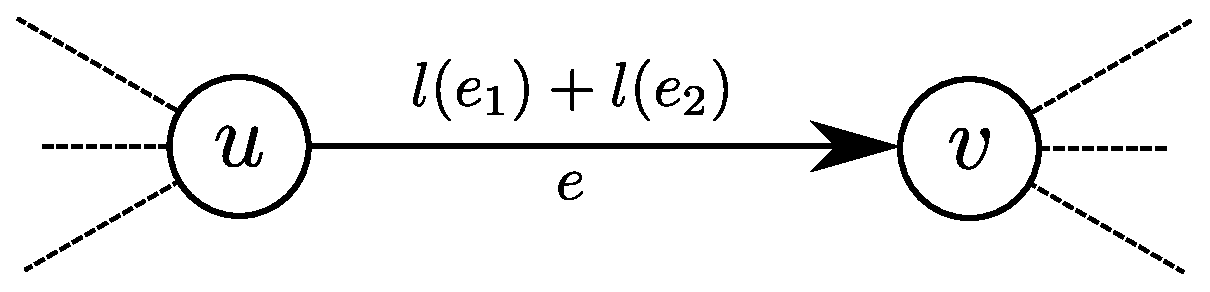
\includegraphics[width=0.95\textwidth]{Content/Pictures/smoothing2.eps}
        \caption{The graph before smoothing $w$}
    \end{subfigure}
    \caption{Smoothing a vertex $w$}
    \label{fig:smoothing}
\end{figure}

\begin{figure}[htbp]
    \centering
    \begin{subfigure}[htbp]{0.45\textwidth}
        \centering
        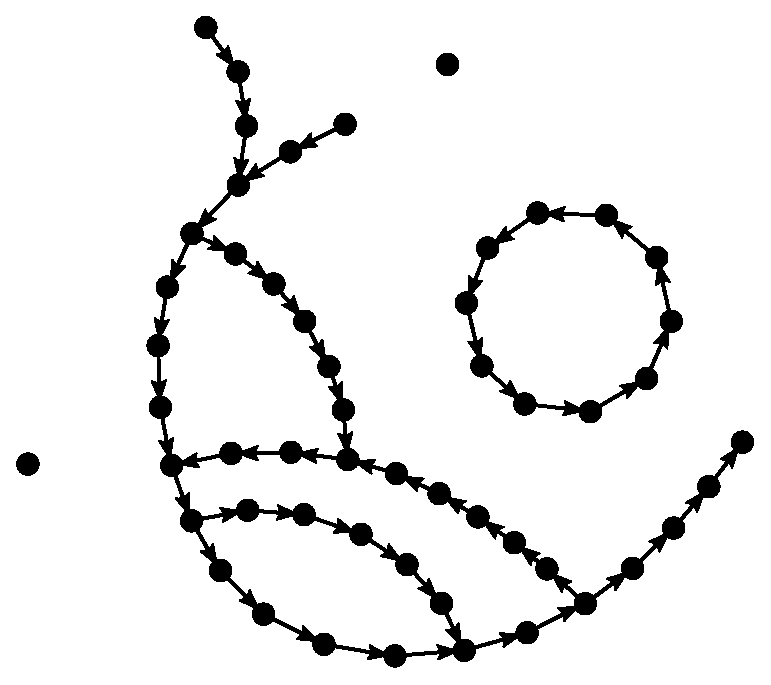
\includegraphics[width=0.90\textwidth]{Content/Pictures/kernel1.eps}
        \caption{$\vec{G}$}
    \end{subfigure}
    \hfill
    \begin{subfigure}[htbp]{0.45\textwidth}
        \centering
        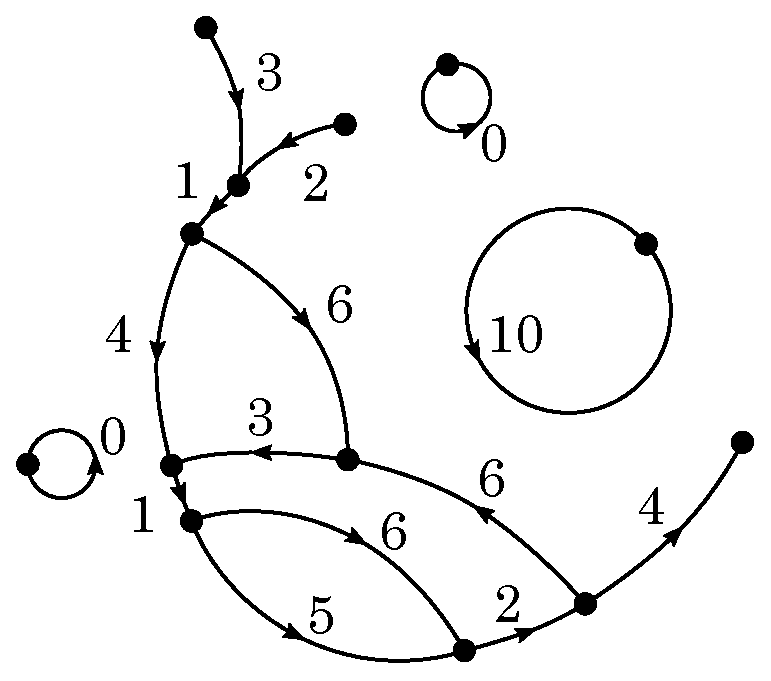
\includegraphics[width=0.90\textwidth]{Content/Pictures/kernel2.eps}
        \caption{$\kernel(\vec{G})$}
    \end{subfigure}
    \caption{An example of a digraph $\vec{G}$ and its kernel $\kernel(\vec{G})$}
    \label{fig:kernel}
\end{figure}

Consider an MDM $M$ and a vertex $w \in M$ with in-degree 1 and out-degree 1 which is not a self-loop. Let $u$ and $v$ be the unique in-neighbour and out-neighbour of $w$ respectively. The MDM obtained by smoothing $w$ is obtained by deleting the edges $e_1$ and $e_2$ such that $r(e_1) = (u, w)$ and $r(e_2) = (w, v)$, then adding an edge $e$ such that $r(e) = (u, v)$ and assigning it length $l(e) = l(e_1) + l(e_2)$. This is illustrated in \cref{fig:smoothing}. Then the kernel of a digraph $\vec{G}$ is obtained by doing the following:
\begin{enumerate}
    \item Assign a length $1$ to each edge.
    \item Iteratively smooth vertices with in-degree 1 and out-degree 1 that are not self-loops until there are none remaining.
    \item Replace all singletons by $\zeroloop$.
\end{enumerate}
Denote the resulting MMD by $\kernel(\vec{G})$. An example is shown in \cref{fig:kernel}.

\subsection{Our results}

Our main result is as follows. Let $C_i(n)$ for $i\geq 1$ be the kernels of the strongly connected components of $\vec{G}_n(\nu)$, listed in decreasing order of size, breaking ties arbitrarily. Complete the list with an infinite repeat of $\zeroloop$. Then, the main theorem is as follows.
\begin{theorem}\label{thm.main}
There exists a sequence $\cC=(\cC_i,i\in \N)$ of random strongly connected MDMs such that, for each $i\geq 1$, $\cC_i$ is either $3$-regular or a loop, and such that 
$$\left(n^{-1/3}C_i(n),i\in \N\right)\overset{d}{\to}\left(\cC_i,i\in \N\right)$$
as $n\to \infty$, with respect to the product $d_{\vec{\cG}}$-topology. The scaling is on lengths in the MDMs.
\end{theorem}
We see here why it is important to consider singletons as loops of length zero. For any fixed $k$, the $k$th largest SCC will not be a singleton with high probability. Therefore no component of our limiting object will be a singleton. Thus we need to pad our SCCs by $\zeroloop$ and consider the kernel of singletons to be $\zeroloop$ so that distance to the limiting object remains finite.

The law of the limit object places our model in the universality class of the directed Erd\H{o}s-Rényi model as studied by \citet{goldschmidtScalingLimitCritical2019}. This is the content of the following Corollary.
\begin{corollary}
Consider $\vec{G}_n(\nu)$, with $\nu$ such that $$\sigma_+=1=\frac{\sigma_{-+}+\nu_-}{\mu}=\frac{\sigma_{-+}+\nu_-}{\mu^2}=1.$$ (Note that this condition is satisfied by $\nu(k^-,k^+)=\nu_1(k^-)\nu_2(k^+)$, with $\nu_i$ the law of a $\operatorname{Poisson}(1)$ random variable.)
Let $(C_i(n), i\geq 1)$ be the strongly connected components of $\vec{G}_n(\nu)$, such that by Theorem \ref{thm.main} there exists $\cC=(\cC_i,i\in \N)$ such that 
$$\left(n^{-1/3}C_i(n),i\in \N\right)\overset{d}{\to}\left(\cC_i,i\in \N\right)$$
as $n\to \infty$, with respect to the product $d_{\vec{\cG}}$-topology. Also consider the directed Erd\H{o}s-R\'enyi model on $n$ vertices, in which any directed edge is present independently with probability $1/n$, which we denote by $\vec{G}(n,1/n)$, and let $(C'_i(n), i\geq 1)$ be the strongly connected components of $\vec{G}_n(\nu)$. Then, also
$$\left(n^{-1/3}C'_i(n),i\in \N\right)\overset{d}{\to}\left(\cC_i,i\in \N\right)$$
as $n\to \infty$, with respect to the product $d_{\vec{\cG}}$-topology. 
\end{corollary}
Moreover, Theorem \ref{thm.main} has the following trivial corollaries, which were previously unknown. 
\begin{corollary}
There exists a random sequence $(\ell_i,i\in \N)\in \R_+^\infty$, such that for $(L^n_i,i\in \N)$ the total lengths in the strongly connected components of $\vec{G}_n(\nu)$ ordered by decreasing length (appended with an infinite repeat of $0$), and for $(S^n_i,i\in\N)$ the number of vertices in the the strongly connected components of $\vec{G}_n(\nu)$ ordered by decreasing size (appended with an infinite repeat of $0$),
$$\left(n^{-1/3}L^n_i,n^{-1/3}S^n_i, i\in \N\right)\overset{d}{\to}\left(\ell_i,\ell_i,i\in \N\right)$$
as $n\to \infty$ in the product topology on $(\R^2)^\infty$. 
\end{corollary}
\begin{corollary}
For $v,w\in \vec{G}_n(\nu)$ such that $v\to w$, let $d(v,w)$ denote the length of the shortest path from $v$ to $w$, and let $$\operatorname{Diam}\left(\vec{G}_n(\nu)\right)=\max\{d(v,w):v\to w\}$$ be the \emph{diameter} of $\vec{G}_n(\nu)$. Then,  $$\operatorname{Diam}\left(\vec{G}_n(\nu)\right)=\Omega(n^{1/3})$$
with high probability.
\end{corollary}


\subsection{Previous work}
The configuration model was introduced by \citet{Bollobas1980} to sample a uniformly random graph with a given degree sequence. For a discussion of the configuration model and proofs of standard results, we refer the reader to \cite[Chapter 7]{hofstadRandomGraphsComplex2017}.

Most results on the configuration model are obtained for models with a deterministic degree sequence. The phase transition for undirected setting was shown in \cite{molloyCriticalPointRandom1995, Molloy1998, Janson2009}. The law of component sizes at criticality and in the critical window were obtained by \citet{Riordan2012} under the assumption that the degrees are bounded. Dhara, van der Hofstad, van Leeuwaarden and Sen showed convergence of the size and surplus edges in the critical window in the finite 3rd moment setting \cite{Dhara2017} and in the heavy-tailed regime \cite{Dhara2020}.  Bhamadi, Dhara, van der Hofstad and Sen obtained metric space convergence in the critical window in \cite{Bhamidi2020}, a result that the authors later improved to a stronger topology in \cite{Bhamidi2020Glmb}. 

Configuration models with a random degree sequence are considered in \cite{josephComponentSizesCritical2014}, \cite{conchon--kerjanStableGraphMetric2020}, and \cite{Donderwinkel2021heightprocess}. \citet{josephComponentSizesCritical2014} showed convergence of the component sizes and surpluses of the large components under rescaling at criticality, both for degree distributions with finite third moments and for the heavy-tailed regime. \citet{conchon--kerjanStableGraphMetric2020} show Gromov-Hausdorff-Prokhorov convergence at criticality in these two regimes. The results in \cite{conchon--kerjanStableGraphMetric2020} in the heavy-tailed regime are extended to the critical window by \citet{Donderwinkel2021heightprocess}. Our techniques are closely related to the techniques introduced in \cite{conchon--kerjanStableGraphMetric2020}. 

Some results have been obtained for other directed graph models. \citet{caoConnectivityGeneralClass2019} consider a class of inhomogeneous directed graphs. Their results include a phase transition for the existence of a giant strongly connected component. This is a generalisation work by \citet{Bloznelis2012}, in which a smaller class of inhomogeneous directed graphs is considered. \citet{Samorodnitsky2016} studied the tails of the degree distribution in the directed preferential attachment model. \citet{goldschmidtScalingLimitCritical2019} studied the directed Erd\H{o}s-R\'enyi model, and were the first to obtain metric space convergence of the strongly connected components of a directed graph. Our methods build on their techniques.

The directed configuration model was first considered by \citet{cooperSizeLargestStrongly2004}. They consider a deterministic degree sequence under a number of conditions, and show that for $\theta$ the expected in-degree of a uniformly chosen vertex, and $\rho$ the expected product of in-degree and out-degree of a uniformly chosen vertex, a phase transition for the strongly connected components occurs at $d=\theta/\rho=1$. They show that for $d<1$, with high probability, all strongly connected components contain $O(\Delta\log(n))$ vertices, for $\Delta$ the maximal degree. On the other hand, for $d>1$, there is a unique strongly connected components that contains a positive proportion of the vertices and also $O(n)$ edges. Their conditions are restrictive, and include finite second moments of both the in- and out-degree of a uniformly chosen vertex, and a bound of size $n^{1/12}/\log(n)$ on the largest degree. Their proofs are based on an algorithm to explore the directed graph. The condition on the largest degree was later relaxed to $O(n^{1/4})$ by \citet{Graf2016}.\myworries{check this is the phase transition}

Recently, Cai and Perarnau have obtained a number of results on the directed configuration model with deterministic degrees. In \cite{caiDiameterDirectedConfiguration2020}, they show, under first and second moment conditions of the degree of a uniformly picked vertex, for $d\neq 1$ (i.e. not at criticality), that the diameter of the model on $n$ vertices, rescaled by $\log(n)$ converges to a constant that they identify. Then, in \cite{caiGiantComponentDirected2020}, they show a law of large numbers for the number of vertices and edges in the largest strongly connected component, under slightly stronger moment conditions, and again not at the critical point. In \cite{cai2021rw}, they study the behaviour of a random walk on a directed configuration model.
 
The emergence of a giant weakly connected component for the directed configuration model with a deterministic degree sequence is discussed in the physics literature by \citet{Kryven2016}. He also studies the distribution of the in- and out-components in \cite{Kryven2017}.

The directed configuration model with random in- and out-degrees is also considered by \citet{Chen2012}, although, importantly, they do not allow for the in- and out-degree of a vertex to be dependent. The authors consider a model in which the in- and out-degrees are two independent sequences of i.i.d.\ random variables drawn from two probability distributions. They propose an algorithm to sample degree sequences that correspond to a simple graph and show the limiting distribution of the degrees generated by this algorithm. 


\subsection{Proof outline}

The techniques we will use to investigate the graph model are a combination of the techniques introduced by Conchon-Kerjan and Goldschmidt in \cite{conchon--kerjanStableGraphMetric2020} and the strategy of Goldschmidt and Stephenson in \cite{goldschmidtScalingLimitCritical2019}. The former work discusses the scaling limit of an undirected uniform graph with i.i.d.\ degrees at criticality, and the latter discusses the scaling limit of the strongly connected components of a directed Erd\H{o}s-Renyi graph at criticality.

To investigate the structure of the strongly connected components of a uniform graph with degree sequence $(\mathbf{D}_1,\dots,\mathbf{D}_n)$, conditional on $\sum_{i=1}^n D^-_i=\sum_{i=1}^n D^+_i$, we will use a version of the configuration model for digraphs that was introduced by \citet{cooperSizeLargestStrongly2004}.

Consider a degree sequence $\vd_1, \ldots, \vd_n$ where $\vd_i = (d_i^-, d_i^+) \in \N \times \N$. We assume 
\begin{equation*}
    \textstyle\sum_{i=1}^n d_i^- = \sum_{i=1}^n d_i^+. 
\end{equation*}
To sample the \emph{directed configuration model} with degree sequence $\vd_1, \ldots, \vd_n$ let $v_1, \ldots, v_n$ be vertices such that $v_i$ has $d_i^-$ in-half-edges and $d_i^+$ out-half-edges. We then pair the in-half-edges and out-half-edges uniformly. This results in a random directed multigraph. The directed configuration model is obtained by This is illustrated in Figure \ref{fig.configuration model}. 

If we then condition on the multigraph being simple, we would get a uniform random digraph on $[n]$ conditioned to have the given degree sequence. This is shown by \citet[P. 10--11]{cooperSizeLargestStrongly2004}. 

To explore the structure of a directed multigraph, we describe an edge-based depth first search procedure (eDFS) in \cref{alg:edfs}. This takes as input a directed multigraph and uses a stack of edges. When the stack is empty, we are at the start of a new out-component and thus pick a new vertex $w$ with probability proportional to its in-degree (this choice simplifies \myworries{insert lemma}). Otherwise we remove the last edge $(v, w)$ off the stack. In both cases, if $w$ has not yet been explored, we add the out-edges from this vertex to the end of the stack of edges (this choice is what makes the exploration depth first).

\myworries{define surplus edges and ordering of vertices}

At each step we also maintain $S^-(k)$ and $S^+(k)$. $S^-(k)$ keeps track of the number of in-edges which we have seen but have not explored the tail of yet at step $k$. $S^+(k)$ is akin to a Lukasiewiescz path. At any given step it is equal to the size of the stack of edges after subtracting the number of fully explored out-components.

We also construct a directed forest for which $S^-(k)$ will be a true Lukasiescz path. At each step of the process we will be examining a vertex $w$. If $w$ has not been explored yet then either we are at the start of a new out-component, in which case we add $w$ to the out-forest, or we are exploring an edge $(v, w)$ where $v$ has already been explored and added to the out-forest, in which case we add $w$ and the edge $(v, w)$ to the out-forest. If $w$ has already been explored we cannot add $(v, w)$ to the out-forest without creating loops. Instead add a dummy vertex to the out-forest and an edge from $v$ to the dummy vertex. We call such dummy vertices purple leafs. This is illustrated in Figure \ref{fig.configuration modeloutforest}. We refer to the out-forest corresponding to the exploration up to time $k$ as $\hat{F}_n(k)$.

\def \exploredvertices {\mathcal V}
\def \explorededges {\mathcal E}
\def \forest {\mathcal F}
\def \edgestack {\mathcal O}
\begin{algorithm}[htbp]
    \SetAlgoLined
    \KwData{A directed multigraph}
    $\exploredvertices \leftarrow$ an empty ordered list of vertices\;
    $\edgestack \leftarrow$ an empty ordered list of edges\;

    $k \leftarrow 0$ \;
    $S^- \leftarrow 0$ \;
    $S^+ \leftarrow 0$ \;
    $\forest \leftarrow$ an empty directed graph\;
    \While(){there exists unexplored vertices of positive in-degree}{
        \eIf(){$\edgestack$ is empty}{
            $w \leftarrow$ a random vertex not in $\exploredvertices$ chosen with prob.\ proportional to $d^-(w)$ \;
        }(){
            $e \leftarrow$ last edge in $\edgestack$ \;
            remove $e$ from $\edgestack$ \;
            $v \leftarrow$ tail of $e$\;
            $w \leftarrow$ head of $e$ \;
            $S^- \leftarrow S^- - 1$ \;
        }
        \eIf(){$w \not \in \exploredvertices$}{
            append $w$ to $\exploredvertices$ \; 
            add the vertex $w$ to $forest$ \;
            \If(){$\edgestack$ is non-empty}{
                add the edge $(v, w)$ to $\forest$\;
            }
            append all out-edges of $w$ to the end of $\edgestack$ in a uniform random order \;
            $S^- \leftarrow S^- + d^-(w)$ \;
            $S^+ \leftarrow S^+ + d^+(w) - 1$ \;
        }{
            add a purple leaf to $\forest$ and and edge from $v$ to the leaf \;
        }
        $k \leftarrow k + 1$ \;
        $S^-_k \leftarrow S^-$ \;
        $S^+_k \leftarrow S^+$ \;
        $\forest_k \leftarrow \forest$ \;
    }
    \caption{The eDFS procedure \label{alg:edfs}}
\end{algorithm}

\begin{figure}
    \centering
    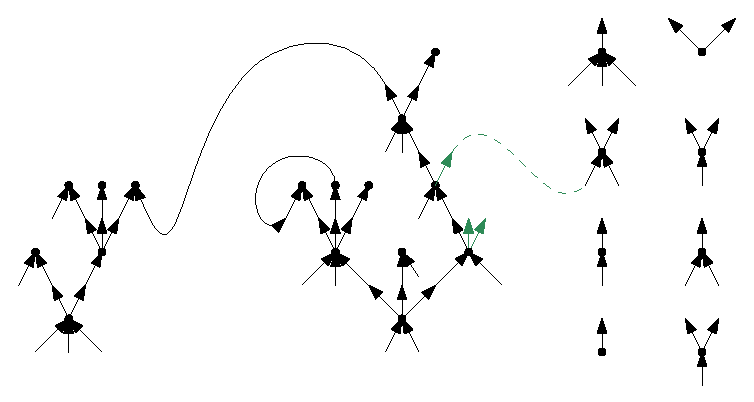
\includegraphics[scale=0.6]{Content/Pictures/configuration_model.eps}
    \caption{The green arrows represent unpaired out-half-edges of vertices that have been visited. One by one, in depth first order, these are paired to a uniform unpaired in-half-edge.}
    \label{fig.configuration model}
\end{figure}

An important motivation for studying the out-forest is the fact that the vertex set of any strongly connected component is contained in one of the components of the out-forest. This is a straightforward property that is further discussed in Lemma \ref{lemma.whatispartofscc}. We have defined the out-forest in such a way that every time step in the exploration corresponds to one vertex in the out-forest. 

A key fact is that the order in which the vertices are discovered does not depend on the position of the purple vertices. Similarly, the position of the purple vertices does not depend on the position of the heads of the surplus edges. Furthermore, we define a necessary condition for a surplus edge to be part of a strongly connected component (see Definition \ref{def.candidate} and Corollary \ref{cor.edgesinSCCs}), and we call these surplus edges \emph{candidates}. The candidates are defined in such a way that whether a purple vertex is a candidate does not depend on the position of the heads of the surplus edges. This allows us to define the following sampling procedure.
\begin{enumerate}
    \item We sample the order of discovery of the vertices in the exploration.
    \item We sample at which time steps a surplus edge is added instead of an edge to an undiscovered vertex, which allows us to define the out-forest $(\hat{F}_n(k),k\geq 1)$. 
    \item We visit the purple vertices in $(\hat{F}_n(k),k\geq 1)$ in depth-first order, and for each vertex we sample whether it corresponds to a candidate.
    \item We visit the tails of the candidates in depth-first order, and for each of them, sample where the head of the corresponding surplus edge is.
\end{enumerate}

\begin{figure}
    \centering
    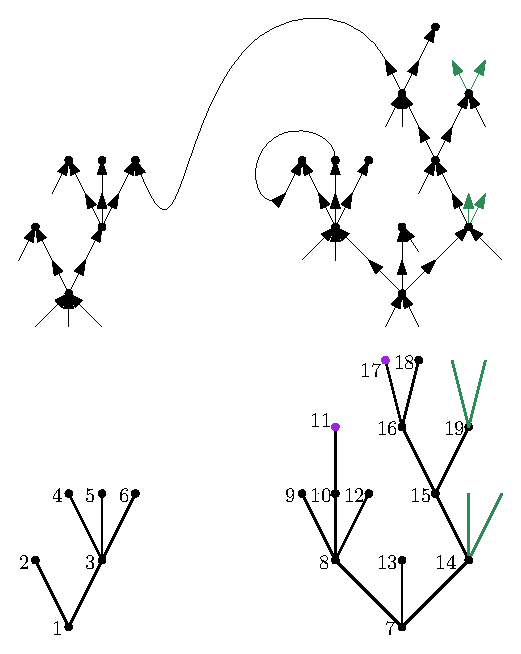
\includegraphics[scale=0.8]{Content/Pictures/configuration_model_out_forest.eps}
    \caption{The out-forest is defined based on the exploration of the digraph. For each surplus edge, we add an extra leaf, which we colour purple. The labels of the vertices correspond to the time step in the exploration at which the vertex is added. The green edges lead to vertices of which the degree and colour have not yet been sampled.}
    \label{fig.configuration modeloutforest}
\end{figure}
Then, our approach is as follows.
\begin{enumerate}
    \item We find the limit under rescaling of the \L ukasiewicz path and height process of $\hat{F}_n(m_n)$ for $m_n=O(n^{2/3})$ conditional on $\sum_{i=1}^n D^-_i=\sum_{i=1}^n D^+_i$ and simplicity of the digraph. (For a definition of the \L ukasiewicz path and height forest, see \cite{AST_2002__281__R1_0}, Chapter 0.)
    \item We show that the positions of the tails of the candidates converge.
    \item We show that the positions of the heads of the candidates converge.
    \item We identify the tails and heads of the candidates, and recover the strongly connected components from the resulting digraph with a cutting procedure. We use a result in \cite{goldschmidtScalingLimitCritical2019} that implies that the cutting procedure converges.
    \item We show that for any $\delta>0$, with high probability, all strongly connected components with length larger than $\delta n^{1/3}$ are contained in the exploration up to time $O(n^{2/3})$. Therefore, we can choose $m_n$ such that, with high probability, we do not miss any large strongly connected components by not considering the exploration beyond time $m_n$. This finishes the proof of the convergence in the product topology.
\end{enumerate}

\subsection{Open problems}
Our work contains the first results on the directed configuration model at criticality, and is the second metric space convergence result for a directed graph model (after the directed Erd\H{o}s-Rényi graph was studied in \cite{goldschmidtScalingLimitCritical2019}), so naturally, there are many interesting unresolved questions.
\begin{enumerate}
    \item The law of our limit object is defined by three parameters that are functions of the (mixed) moments of the degree distribution. Does a different choice of parameters always give a different limit distribution? If so, are the laws absolutely continuous to one another?
    \item Our methods show that the diameter of the configuration model at criticality is  $\Omega(n^{1/3})$, which is in contrast with the off-critical cases (for deterministic degrees), in which the diameter is $O(\log(n))$ \cite{caiDiameterDirectedConfiguration2020}. We believe that the diameter is in fact exactly $O(n^{1/3})$. Goldschmidt and Maazoun are working on this question for the directed Erd\H{o}s-Rényi graph at criticality. 
    \item In \cite{goldschmidtScalingLimitCritical2019}, the authors show convergence of the sequence of SCCs in the $\ell_1$-sense, which is stronger than the product topology as considered by us. This for example implies that for the directed Erd\H{o}s-Rényi graph, the total length in the SCCs converges in distribution to some finite number. Also for undirected configuration models, there are no results that show metric space convergence in a topology on the sequence of components that is stronger than the product topology \cite{Bhamidi2020}\cite{conchon--kerjanStableGraphMetric2020}\cite{Bhamidi2020Glmb}.
     \item We conjecture that, just like the directed Erd\H{o}s-Rényi graph \cite{goldschmidtScalingLimitCritical2019}, the directed configuration model gives rise to a critical window, that in some sense interpolates between subcritical and supercritical models. It would be interesting to adapt our methods to the critical window.
     \item We plan to extend our understanding of the strongly connected components by studying the directed graphs that they are embedded in. A first step would be to study all vertices that can be reached from the non-trivial strongly components. This would illuminate connections between the strongly connected components and expose the fractal structure of the directed graph, which is not observed when only studying the strongly connected components themselves.
    \item Another natural next step is to study the model under weaker moment conditions. The first condition to eliminate is $\E\left[(D^-)^i(D^+)^j\right]$ for $\{i,j\}=\{1,3\}$, which would in some sense makes the identifications less uniform on the ancestral lines. We have reason to believe that this would place the model in  a different universality class, but further research is needed to confirm this. Also the heavy-tailed case is not well-understood, but given our results, it is natural to expect the limit object to be embedded in a tilted stable tree as defined in \cite{conchon--kerjanStableGraphMetric2020}. Moreover, one could define hybrid models by letting the tail-behaviour of the in- and out-degrees be different. 
    \item We conjecture that the inhomogeneous directed random graph model under suitable conditions is part of the same universality class as the directed Erd\H{o}s-Rényi graph \cite{goldschmidtScalingLimitCritical2019} and $\vec{G}_n(\nu)$. We believe that our methods and the methods of \cite{goldschmidtScalingLimitCritical2019} can be adapted to obtain a metric space scaling limit for the inhomogeneous directed random graph model. 

\end{enumerate}

